\scanpage{83}
\mspage{82}
Plus généralement, on peut prendre deux ensembles ordonnés $I,I'$, \deleted{Prendre le} \inserted{sans extrémités} (totalement si on veut) prendre le produit $I\times I'$, et rajouter un plus petit et un plus grand élément (``origine'' et ``extrémité''), \unsure{ceci pour former} $J$
\[
z=(x,x')\in J^{\circ}=I\times I'
\]
on voit que
\[
A_z=\{z\}
\]
est un \unsure{ensemble} support, car \unsure{ce sera} le cosupport de l'ens des \deleted{\unsure{parties}} \inserted{\unsure{Antos|Autos}} de la forme
\[
\deleted{\unsure{J_{\geq z'}}}\qquad
\begin{aligned}
[z'',1]&\quad\text{pour }z''>z\\
[0,z']&\quad\text{pour }z'<z
\end{aligned}
\]
Considérons la fonction-support \deleted{qui \unsure{prend}} \inserted{naturelle} à valeurs dans $I\amalg I'\amalg\{0\}\amalg\{1\}$
\[
\begin{aligned}
|z|&=\{x,x'\}\qquad\text{si }z=\unsure{\{x,x'\}|(x,x')}\quad x\in I,\\
|\deleted{\unsure{z}}0|&=\{0\}\\
|1|&=\{1\}
\end{aligned}
\]
Le cosupport de $A_z$ est
\[
B_z=\{z'\in J\mid z'<z\text{ ou }z'>\deleted{\unsure{J}}z\}
\]
\uline{Et on} voit tout de suite que
\[
\deleted{\unsure{B_{z_1}\cap B_{z_2}=}}\qquad
|B_z|=J\smallsetminus|z|\qquad\text{comme il se doit}
\]
Mais si $z_1,\unsure{z_2^{+}|z_2^{*}|z_2}$ ne sont pas comparables, on aura
\[
|B_{z_1}\cap B_{z_2}|\subsetneq|B_{z_1}|\cap|B_{z_2}|
\]
\figure{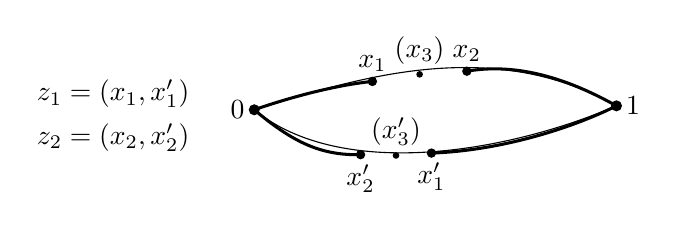
\begin{tikzpicture}[x=1cm,y=1cm]
\draw (0,0) .. controls (1.3,.4) and (3,.95) .. (4.6,.05);
\draw (0,0) .. controls (1.1,-.9) and (3.2,-.55) .. (4.6,.05);
\draw[line width=1.1pt] (0,0) .. controls (.4,.14) and (1,.31) .. (1.5,.36);
\draw[line width=1.1pt] (2.7,.49) .. controls (3.45,.62) and (4.15,.3) .. (4.6,.05);
\draw[line width=1.1pt] (0,0) .. controls (.5,-.42) and (.85,-.58) .. (1.35,-.57);
\draw[line width=1.1pt] (2.25,-.55) .. controls (3.1,-.52) and (4,-.25) .. (4.6,.05);
\fill (0,0) circle (2pt) node[left] {$0$};
\fill (4.6,.05) circle (2pt) node[right] {$1$};
\fill (1.5,.36) circle (1.7pt) node[above] {$x_1$};
\fill (2.1,.45) circle (1.2pt) node[above] {$(x_3)$};
\fill (2.7,.49) circle (1.7pt) node[above] {$x_2$};
\fill (1.35,-.57) circle (1.7pt) node[below] {$x'_2$};
\fill (1.8,-.58) circle (1.2pt) node[above] {$(x'_3)$};
\fill (2.25,-.55) circle (1.7pt) node[below] {$x'_1$};
\node[anchor=east] at (-.7,.2) {$z_1=(x_1,x'_1)$};
\node[anchor=east] at (-.7,-.35) {$z_2=(x_2,x'_2)$};
\end{tikzpicture}}
Il manque $\mathopen{]}z_1,z_2\mathclose{[}$ sur $I$ et $\mathopen{]}z'_2,z'_1\mathclose{[}$ sur $I'$

ou dualement
\[
[x_1,x_2]\cup[x'_2,x'_1]=|A_{z_1}\vee A_{z_2}|\supsetneq|A_{z_1}|\cup|A_{z_2}|=\{x_1,x_2,x'_1,x'_2\}
\]
